\chapter{Pravidla deskové hry}
Logic je desková hra pro dva hráče \cite{Logic_pravidla}. Jeden hráč určí hledanou kombinaci, dále bude označován jako 
hráč~A, a~druhý tuto kombinaci za pomoci logických úvah a~vyhodnocení hráčem~A~hledá, dále bude označován jako hráč~B.

Hráči si určí herní pozice. Hráč~A~vybere barevné kolíky dle libosti a~následně je v~určitém pořadí vloží do zadávacího pole. Zadání zakryje
stříškou, aby tuto
kombinaci spoluhráč neviděl. Hráč~B~se po tuto dobu nedívá. Hráč~B~následně zvolí libovolnou kombinaci barev a~jejich pozic. Po 
ukončení tahu nechá
hráče~A,~aby jeho tah vyhodnotil. Hráč~A~vyhodnotí tah následujícím způsobem. Pokud hráč~B~vložil správnou barvu na správnou pozici, tak vloží 
do vyhodnocovací sekce černý kolík. Pokud vložil barvu, která se v~zadání vyskytuje, ale vložil ji na nesprávnou pozici, tak vloží bílý kolík.
Pokud zůstanou některé pozice neobsazené, tak to znamená, že se dané barvy v~zadání nevyskytují. 
Vyhodnocovací kolíky umisťuje od kraje, nejprve černé a~pak bílé, aby hráči~B~nebylo jasné, kterých hracích kolíků se vyhodnocení 
týká \cite{Logic_pravidla}.
Poté začne hráč~B~na základě vyhodnocení a~svých všech předchozích tahů hledat správnou kombinaci.

Hráč~B~má maximálně 10~pokusů na zjištění správné kombinace. Po skončení hry hráč~A~odkryje stříšku a~ukáže hledanou kombinaci, aby mohlo dojít
k~případné kontrole. Hra skončí po určení správné kombinace, nebo po vypotřebování všech pokusů.

Hru lze hrát ve více variantách. Hráči se mohou domluvit, zda zadání může, nebo nesmí obsahovat volnou pozici. Dále se může hra lišit v~délce hledané 
kombinace.

\begin{figure}[!h]
  \begin{center}
    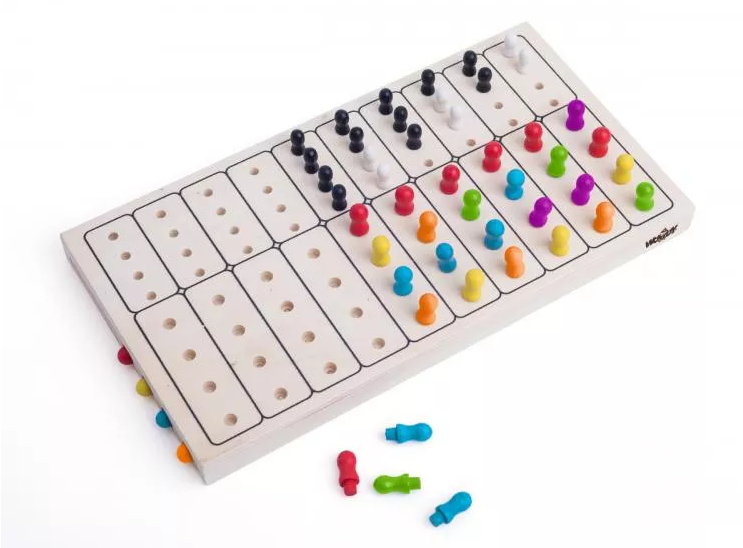
\includegraphics[scale=0.6]{obrazky/Logic_deskovka.png}
  \end{center}
  \caption[Desková hra Logic \cite{Logic_deskovka}]{Desková hra Logic \cite{Logic_deskovka}.}
\end{figure}

\chapter{Návrh elektroniky}
V~následující kapitole budou rozebrány všechny komponenty DPS Elektronické hry Logic. Návrh se skládá z~řídicí elektroniky, 
napájení, herních prvků a~dalších potřebných komponent.

\begin{figure}[!h]
  \begin{center}
    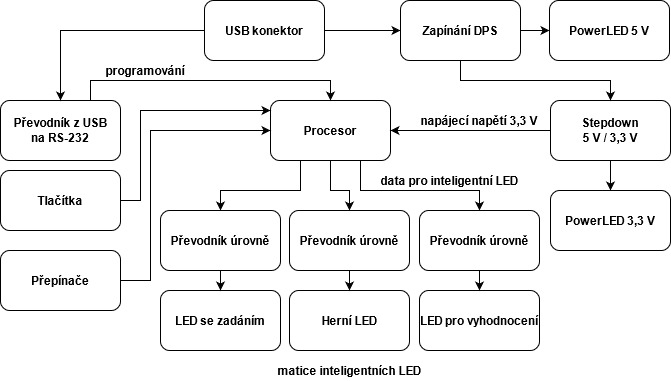
\includegraphics[scale=0.6]{obrazky/v2_blokove_schema.jpg}
  \end{center}
  \caption[Blokové schéma elektroniky]{Blokové schéma elektroniky.}
\end{figure}    

\section{Řídicí elektronika} \label{Ridici_elektronika}
Jako řídicí elektronika byl vybrán mikrokontrolér ESP32-PICO-D4. Hlavním důvodem pro výběr tohoto mikrokontroléru bylo, že je téměř totožný 
jako ESP32-WROOM, se 
kterým mám dlouhodobé zkušenosti. Tento mikrokontrolér má veškeré periferie, které jsou pro výrobu této hry zapotřebí. 

Mikrokontrolér ESP32-PICO také podporuje Arduino framework, díky kterému bylo programování značně zjednodušeno.

Mikrokontrolér ESP32-PICO obsahuje \cite{PICO_datasheet}: 
\begin{itemize}
    \item modul WiFi,
    \item modul Bluetooth, 
    \item 32~GPIO pinů, 
    \item dvoujádrový 32bitový procesor Xtensa LX6,
    \item 520~kB~SRAM, 
    \item 4~MB~FLASH. 
  \end{itemize}

  Napájecí napětí tohoto mikrokontroléru je 3,0--3,6~V~a průměrný odběr proudu je 80~mA \cite{PICO_datasheet}. Mikrokontrolér ESP32-PICO má 
  vyvedeno 32~GPIO pinů, které je 
  možno softwarově nastavit jako vstupní nebo výstupní. Na tyto piny lze poté připojit různá zařízení. Vstupním senzorem může 
  být typicky tlačítko a~výstupním indikátorem např.~LED. Tato zařízení zprostředkovávají komunikaci mezi mikrokontrolérem a~okolním 
  světem.

  \begin{figure}[!h]
    \begin{center}
      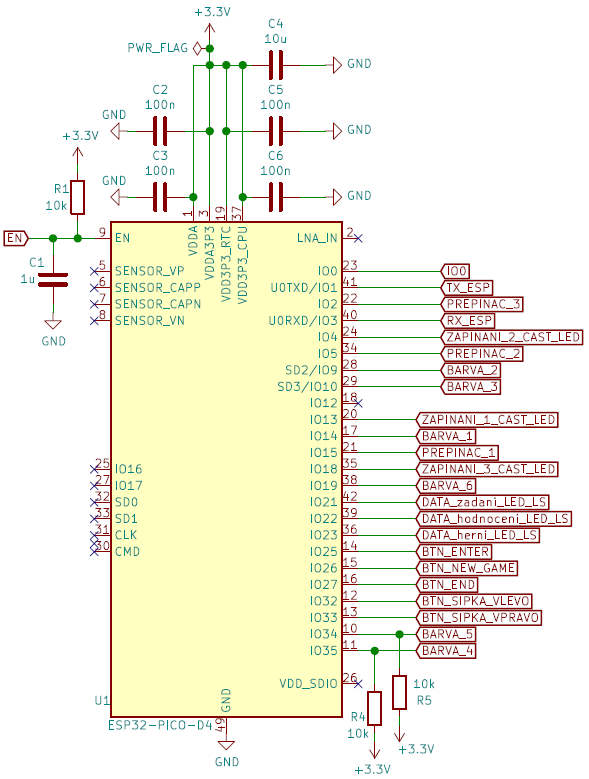
\includegraphics[scale=0.5]{obrazky/ESP32_PICO_schema.png}
    \end{center}
    \caption[Schéma zapojení mikrokontroléru ESP32-PICO \cite{PICO_datasheet}]{Schéma zapojení mikrokontroléru ESP32-PICO \cite{PICO_datasheet}.}
  \end{figure}

  Vstupně-výstupní piny IO16 a~IO17 nemohou být použity, protože ESP32-PICO má na těchto pinech připojenou flash paměť \cite{PICO_datasheet}.
  Pokud by na tento pin bylo připojeno nějaké zařízení, tak by mikrokontrolér ztratil přístup ke své paměti.

  Vstupně-výstupní piny IO02, IO05, IO12 a~IO15 slouží jako konfigurační piny při spouštění nebo resetu mikrokontroléru ESP32-PICO. Slouží například k~výběru
  paměti, ze které se program mikrokontroléru ESP32-PICO načítá. Při resetu musí být tyto piny ve správné konfiguraci. Pin MTDI je GPIO12 a~pin MTDO je pin 
  GPIO15 \cite{PICO_datasheet}.

  \begin{table}[!h]
    \caption{Konfigurační piny \cite{PICO_datasheet}.}
    \begin{center}
      \begin{tabular}{|c|c|c|c|c|c|}
      \hline
      \rowcolor[HTML]{9B9B9B} 
      \multicolumn{6}{|c|}{\cellcolor[HTML]{9B9B9B}{\color[HTML]{000000} Napětí interního LDO (VDD\_SDIO)}} \\ 
      \hline
      \rowcolor[HTML]{C0C0C0} 
      Pin & Výchozí & \multicolumn{2}{c|}{\cellcolor[HTML]{C0C0C0}3.3~V} & \multicolumn{2}{c|}{\cellcolor[HTML]{C0C0C0}1.8~V} \\ 
      \hline
      MTDI & Pulldown  & \multicolumn{2}{c|}{0}   & \multicolumn{2}{c|}{1}  \\ 
      \hline
      \rowcolor[HTML]{9B9B9B} 
      \multicolumn{6}{|c|}{\cellcolor[HTML]{9B9B9B}{\color[HTML]{000000} Startovací sekvence}}  \\ 
      \hline
      \rowcolor[HTML]{C0C0C0} 
      Pin  & Výchozí & \multicolumn{2}{c|}{\cellcolor[HTML]{C0C0C0}Načtení programu z SPI}   & \multicolumn{2}{c|}{\cellcolor[HTML]{C0C0C0}Načtení programu z interní paměti} \\ 
      \hline
      GPIO0  & Pullup  & \multicolumn{2}{c|}{1} & \multicolumn{2}{c|}{0} \\ 
      \hline
      GPIO2  & Pulldown & \multicolumn{2}{c|}{Nezáleží}  & \multicolumn{2}{c|}{0}  \\ 
      \hline
      \rowcolor[HTML]{9B9B9B} 
      \multicolumn{6}{|c|}{\cellcolor[HTML]{9B9B9B}Povolení/Zakázání zobrazení ladicího protokolu U0TXD v průběhu načítání} \\ 
      \hline
      \rowcolor[HTML]{C0C0C0} 
      Pin  & Výchozí  & \multicolumn{2}{c|}{\cellcolor[HTML]{C0C0C0}U0TXD aktivní} & \multicolumn{2}{c|}{\cellcolor[HTML]{C0C0C0}U0TXD neaktivní} \\ 
      \hline
      MTDO & Pullup & \multicolumn{2}{c|}{1}  & \multicolumn{2}{c|}{0} \\ 
      \hline
      \rowcolor[HTML]{9B9B9B} 
      \multicolumn{6}{|c|}{\cellcolor[HTML]{9B9B9B}Časování SDIO periferního zařízení} \\ 
      \hline
      \rowcolor[HTML]{C0C0C0} 
      {\color[HTML]{000000} Pin} & {\color[HTML]{000000} Výchozí} & {\color[HTML]{000000} \begin{tabular}[c]{@{}c@{}} $\downarrow$ vzorkování\\ $\downarrow$ výstup\end{tabular}} & {\color[HTML]{000000} \begin{tabular}[c]{@{}c@{}} $\downarrow$ vzorkování\\ $\uparrow$ výstup\end{tabular}} & {\color[HTML]{000000} \begin{tabular}[c]{@{}c@{}} $\uparrow$ vzorkování\\ $\downarrow$ výstup\end{tabular}} & {\color[HTML]{000000} \begin{tabular}[c]{@{}c@{}} $\uparrow$ vzorkování\\ $\uparrow$ výstup\end{tabular}} \\ 
      \hline
      MTDO  & Pullup  & 0    & 0   & 1  & 1 \\ 
      \hline
      GPIO5  & Pullup  & 0  & 1 & 0  & 1 \\ 
      \hline
      \end{tabular}  
    \end{center}
  \end{table}  

  Vstupně-výstupní piny IO34 a~vyšší jsou pouze vstupní \cite{PICO_datasheet}. Vstupní piny nemají softwarově zapojitelný pullup rezistor. 
  Pokud je tedy zapotřebí pullup rezistor, musí se fyzicky zapojit.
  
  \section{Napájení}
  Napájení probíhá před USB konektor. V~dnešní době jsou 2~nejpoužívanější konektory – USB Micro a USB-C. Proto byly použity oba USB konektory. 
  Deska plošného spoje nepodporuje funkci Quick Charge ani Power Delivery. Může být napájena pouze napětím 5~V. Přítomnost jiného napětí není žádoucí. 
  Konektor USB-C je tedy funkčně zapojen totožně jako USB~Micro a~oba konektory jsou na DPS pouze kvůli jejich tvarům. 
  
  \begin{figure}[!h]
    \begin{center}
      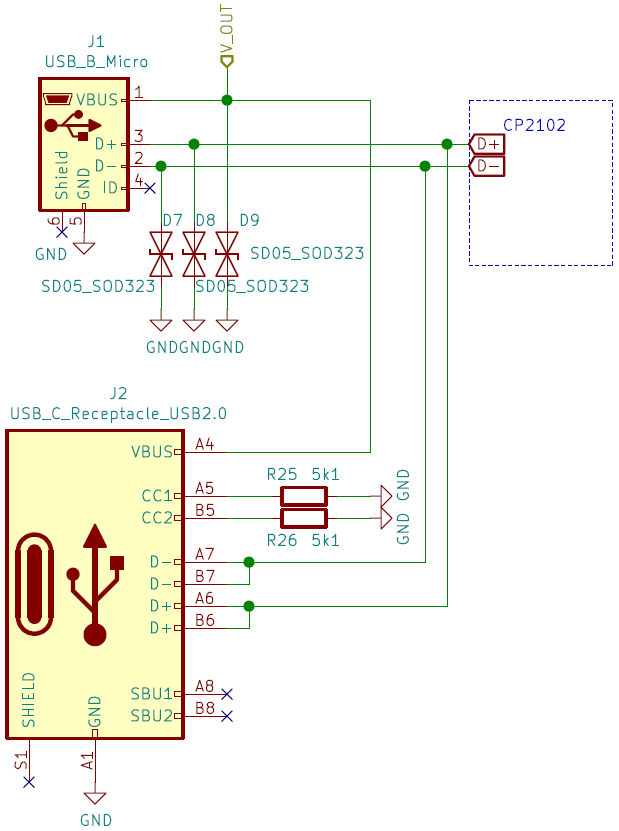
\includegraphics[scale=0.5]{obrazky/Obe_USB_schema.png}
    \end{center}
    \caption[Schéma zapojení USB konektorů \cite{USB-C}]{Schéma zapojení USB konektorů \cite{USB-C}.}
  \end{figure}

  \section{Snižující měnič napájecího napětí}
  Mikrokontrolér ESP32-PICO má napájecí napětí 3,3~V. Napětí z~powerbanky přes USB je 5~V. Proto je tedy zapotřebí zapojit 
  měnič pro snížení napětí, který bude vytvářet z~napájecího napětí 5~V~napájecí napětí 3,3~V~pro mikrokontrolér ESP32-PICO.

  Jako měnič byl zvolen čip SY8105. Tento čip byl vybrán podle projektu RB0005-UniversalStepDown \cite{UniversalStepDown}. 
  V~tomto projektu zapojení funguje bezproblémově, a~proto bylo rozhodnuto toto zapojení použít v~této práci. 

  Čip SY8105 má napájecí napětí 4,5--18~V~a jeho maximální výstupní proud může dosahovat až 5~A.

  Výstupní napětí zapojení čipu SY8105 je závislé na poměru rezistorů R11~a~R12 \cite{SY8105_datasheet}. 
  Hodnota rezistoru R11 byla zvolena 160~k$\Omega$. Hodnota rezistoru R12 byla dopočítána dle:

  \begin{equation} 
    R_{12}~=~\frac{0,6}{U_{OUT}-0,6}~\cdot~R_{11}~=~\frac{0,6}{3,3-0,6}~\cdot~160\cdot10^3~=~35,555~\:k\Omega. 
    \quad \quad \quad \cite{SY8105_datasheet}
  \label{eq:R12}
  \end{equation}

  Hodnota rezistoru R12 byla zvolena nejbližší z~vyráběné rezistorové řady E24, tudíž 36~k$\Omega$ \cite{Rezistorova_rada}. Hodnota 
  rezistoru se musí co nejvíce blížit vypočítané hodnotě, aby výstupní napětí nebylo příliš odlišné od požadovaného. Proto nebyl
  zvolen rezistor z~častěji používaných řad E6 ani E12. Hodnota rezistoru z~těchto řad by se již příliš odchylovala od vypočítané.

  \begin{figure}[!h]
    \begin{center}
      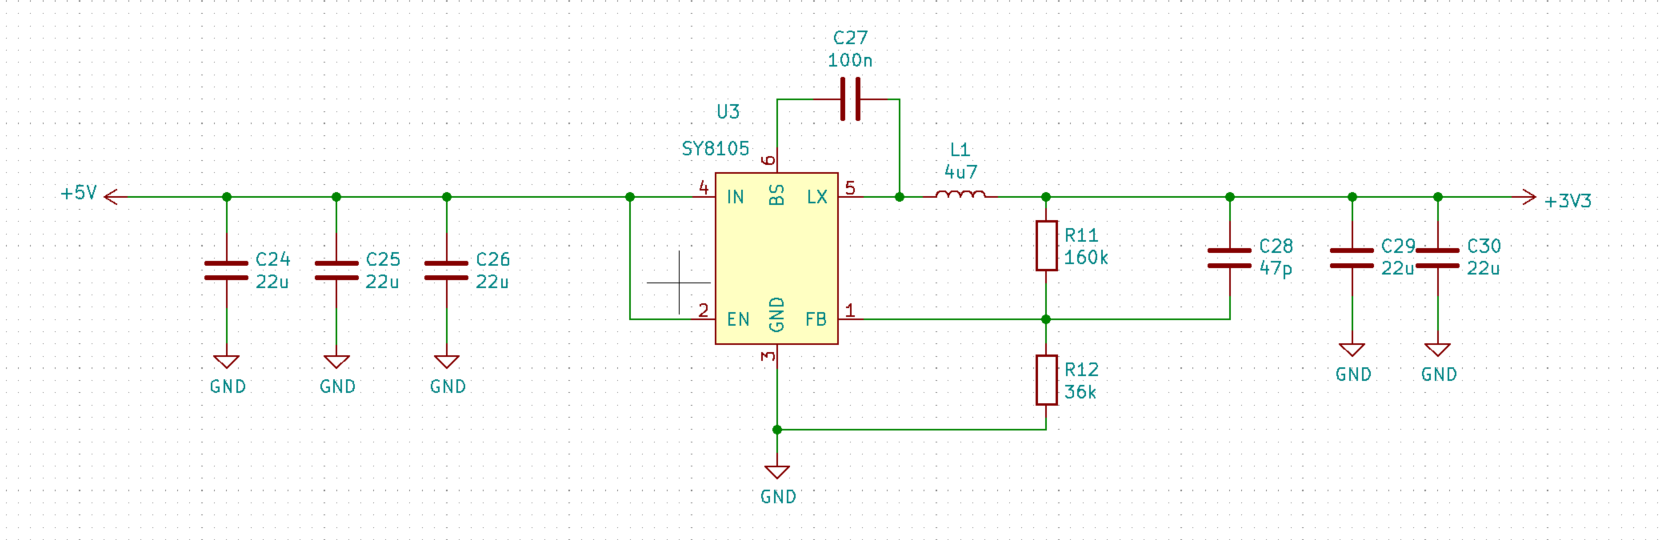
\includegraphics[scale=0.4]{obrazky/SY8105_schema.png}
    \end{center}
    \caption[Schéma zapojení čipu SY8105 \cite{SY8105_datasheet}]{Schéma zapojení čipu SY8105 \cite{SY8105_datasheet}.}
  \end{figure}

  \section{Převodník z~USB na RS-232}
  Mikrokontrolér ESP32-PICO používá jako komunikační rozhraní linku RS-232. Programování ale probíhá přes USB konektor, který toto rozhraní
  nemá. Proto bylo potřeba použít převodník z~USB na rozhraní RS-232.
  
  \begin{figure}[!h]
    \begin{center}
      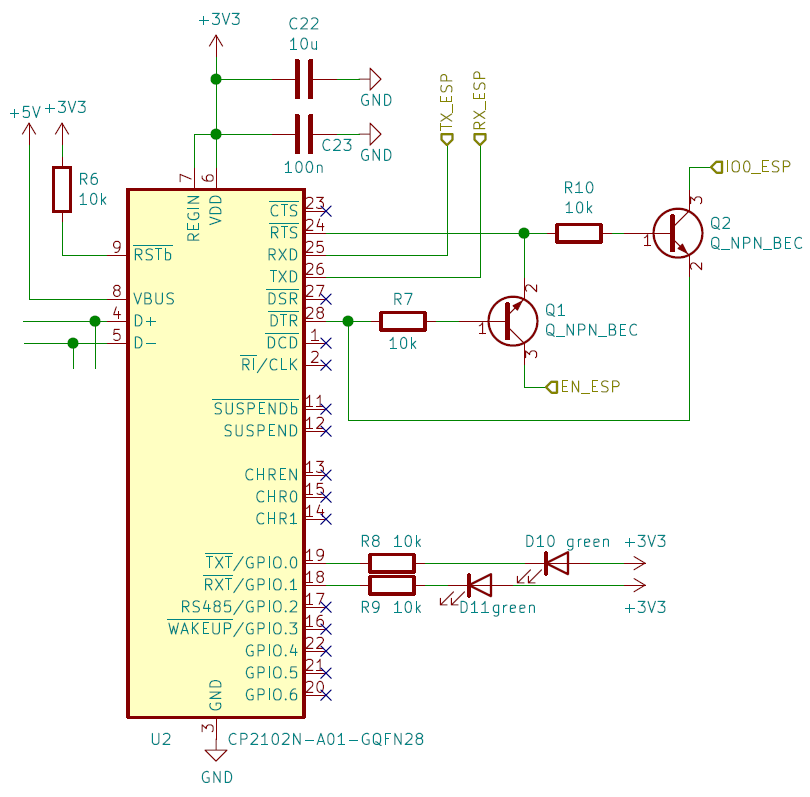
\includegraphics[scale=0.5]{obrazky/CP2102_schema.png}
    \end{center}
    \caption[Schéma zapojení převodníku z~USB na RS-232 \cite{Devkit_schema}]{Schéma zapojení převodníku z~USB na RS-232 \cite{Devkit_schema}.}
  \end{figure}

  Velkou inspirací při výběru součástek byl kit ESP32-DEVKITC \cite{Devkit_schema}. Tento kit obsahuje ESP32-WROOM a~také převodník
  z~USB na RS-232. Na tomto kitu je převodník realizován čipem CP2102. Mikrokontrolér ESP32-WROOM a~ESP32-PICO se liší pouze v~drobnostech, 
  proto byl převodník CP2102 použit i~při návrhu převodníku u~Elektronické hry Logic.  Tento čip zároveň převádí logiku 
  z~0--5~V~na logiku 0--3,3~V~\cite{CP2102_datasheet}. 

 Čip CP2102 má napájecí napětí 3--3,6~V a~jeho typickým proudovým odběrem je 9,5~mA.

  Čip CP2102 dokáže komunikovat velkým množstvím komunikačních rychlostí (300, 9600, 19200, 38400, 115200, 256000~Bd, atd) 
  \cite{CP2102_datasheet}. Komunikační rychlost se nastavuje během konfigurace COM portu v~počítači \cite{CP2102_datasheet}.

  Z~USB jsou signály D+~a~D- připojeny k~čipu CP2102. Tento čip signál z~USB převede na signály RX~a~TX, které mají výstup 
  na pinech RXD~a~TXD. Následně jsou tyto signály připojeny k~mikrokontroléru ESP32-PICO. Signály RX~a~TX musí být překříženy. To znamená, že RX CP2102
  je připojeno na TX ESP32-PICO a~TX CP2102 je připojeno na RX ESP32-PICO. 

  Elektroluminiscenční diody~D10~a~D11 slouží k~indikaci komunikace s~mikrokontrolérem ESP32-PICO. Pokud je do mikrokontroléru nahráván program, tak LED~D10~a~D11 
  blikají.

  \begin{figure}[!h]
      \begin{center}
        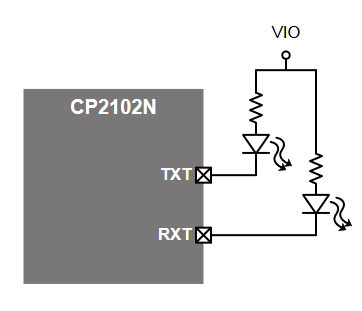
\includegraphics[scale=0.35]{obrazky/CP2102_LED.png}
      \end{center}
      \caption[Zapojení LED pro indikaci komunikace čipu CP2102 s~mikrokontrolérem ESP32-PICO \cite{CP2102_datasheet}]{Zapojení LED pro indikaci 
      komunikace čipu CP2102 s~mikrokontrolérem ESP32-PICO \cite{CP2102_datasheet}.}
  \end{figure}

  \newpage
  \section{Herní prvky}
  Herními prvky Elektronické hry Logic jsou inteligentní LED typu WS2812C. Tento typ inteligentních LED je určen pro přenosná 
  zařízení, protože mají oproti obdobným LED velmi nízkou spotřebu. Jsou také plně kompatibilní s~typem WS2812B \cite{WS2812C_datasheet}. K~těmto 
  inteligentním LED existují knihovny, které usnadňují softwarovou práci s~nimi.

  \begin{figure}[!h]
    \begin{center}
      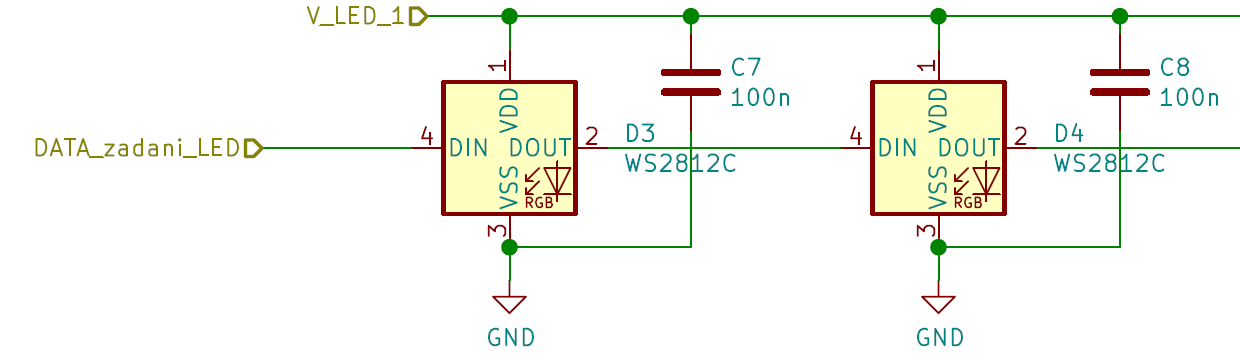
\includegraphics[scale=0.5]{obrazky/2_LED_WS2812C.png}
    \end{center}
    \caption[Zapojení inteligentních LED WS2812C \cite{WS2812C_datasheet}]{Zapojení inteligentních LED WS2812C \cite{WS2812C_datasheet}.}
  \end{figure}

  Každá inteligentní LED má v~sobě procesor, který slouží pro zpracování dat. 
  Inteligentní LED WS2812C se zapojují za sebou přes piny DATA~IN a~DATA~OUT. Každá inteligentní LED převezme data z~pinu 
  DATA~IN, která jsou pro ni určena, a~zbytek pošle ven přes pin DATA~OUT. K~pinu DATA~OUT je připojen pin DATA~IN další inteligentí LED. 

  \begin{table}[!h]
    \caption{Parametry inteligentních LED WS2812C \cite{WS2812C_datasheet}}
    \begin{center}
        \begin{tabular}{|c|c|}
            \hline
            {\cellcolor[HTML]{C0C0C0}Napájecí napětí} & 3,5--5,3~V~\\
            \hline
            {\cellcolor[HTML]{C0C0C0}Výstupní napětí} & (VDD~-~0,5)--(VDD~+~0,5)~V~\\
            \hline
            {\cellcolor[HTML]{C0C0C0}Typický odběr proudu}  & 5~mA \\
            \hline
            {\cellcolor[HTML]{C0C0C0}Klidový odběr proudu}  & 0,3~mA \\
            \hline
        \end{tabular}    
    \end{center}
  \end{table}

  Ke každé inteligentní LED je připojen mezi napájecí napětí a~GND filtrační kondenzátor, aby LED svítily kontinuálně 
  a~nedostal se jim na napájení žádný šum \cite{WS2812C_datasheet}.

  \subsection{Rozdělení}
  Inteligentní LED jsou rozděneny do tří skupin. Skupina inteligentních LED pro zadání, skupina inteligentních LED pro herní pole 
  a~skupina inteligentních LED pro zobrazení vyhodnocení tahu.
  Skupina inteligentních LED pro zadání obsahuje 4~LED a~skupiny pro herní pole a~pro vyhodnocení každá 40~LED.

  \subsection{Převodník úrovně}
  Inteligentní LED WS2812C pracují s~logikou 0--5~V. Mikrokontrolér ESP32-PICO pracuje s~logikou 0--3,3~V. 
  Z~tohoto důvodu byl mezi mikrokontrolér a inteligentní LED, na datový signál pro inteligentní LED, zapojen převodník úrovně, 
  tzv.~level shifter. 
  
  Převodník je realizován MOSFET tranzistorem a~dvěma pullup rezistory. Jeden rezistor je připojen k~napájecímu napětí 3,3~V a~druhý
  k~napájecímu napětí 5~V. Jedná se o~nejjednodušší způsob převodníku úrovně směrem nahoru. Tento způsob umožňuje komunikaci oběma směry. 
  Tranzistor MOSFET byl zvolen pro téměř nulovou spotřebu, narozdíl od bipolárních tranzistorů. Tranzistory MOSFET jsou také rychlejší 
  než bipolární tranzistory, takže způsobí menší zkreslení signálu. 

  \begin{figure}[!h]
    \begin{center}
      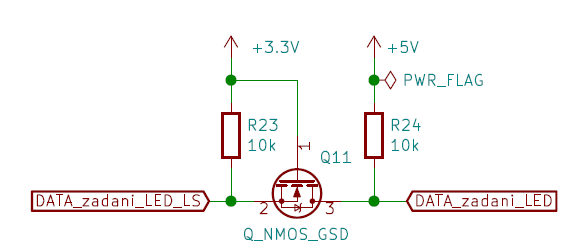
\includegraphics[scale=0.85]{obrazky/level_shifter.png}
    \end{center}
    \caption[Zapojení převodníků úrovně]{Zapojení převodníku úrovně.}
  \end{figure}

  Pokud jsou obě zařízení v~klidu (nekomunikují), tak je tranzistor zavřený a~pullup rezistory zajišťují, že na pinu mikrokontroléru
  i~inteligentní LED je logická~1. Pro mikrokontrolér ESP32-PICO je to tedy 3,3~V a~pro inteligentní LED WS2812C je to 5~V. Jakmile započne
  mikrokontrolér komunikaci, to znamená, že svůj stav přepne do stavu logické nuly (0~V), tak rozdíl mezi gate a~source tranzistoru stoupne a~na 
  výstupu tranzistoru bude také logická nula (0~V). Pokud by komunikace mohla probíhat i~naopak (inteligentní LED by odesílala data do
  mikrokoltroléru), tak by byl princip totožný. 

  \subsection{Zapínání napájení}
  Deska plošného spoje je navrhována pro přenosnou aplikaci, a~proto je potřeba zajistit její co nejnižší odběr. 

  Inteligentní LED WS2812C mají spotřebu 0,3~mA ve vypnutém stavu \cite{WS2812C_datasheet}. I~takto nízká spotřeba je  pro přenosnou aplikaci 
  nežádoucí. Připojení
  napájení inteligentním LED je tedy spínáno. Proto je herní pole dohromady
  s~vyhodnocovacími LED rozděleno na 3~části. Tyto 3~části mají rozděleno napájení, které je postupně softwarově zapínáno dle potřeby. 
  Do první části patří inteligentní LED se zadáním a~první 4~čtveřice inteligentních LED 
  z~herního pole a~z~vyhodnocení. Do druhé části patří další 3~čtveřice inteligentních LED z~herního a~vyhodnocovacího pole. 
  Do třetí části patří poslední 3~čtveřice inteligentních LED z~herního a z~vyhodnocovacího pole.

  Ke spínání slouží obvody s~MOSFET tranzistory. Tranzistory MOSFET byly zvoleny pro jejich téměř nulovou spotřebu, narozdíl od 
  bipolárních tranzistorů. 

  \begin{figure}[!h]
    \begin{center}
      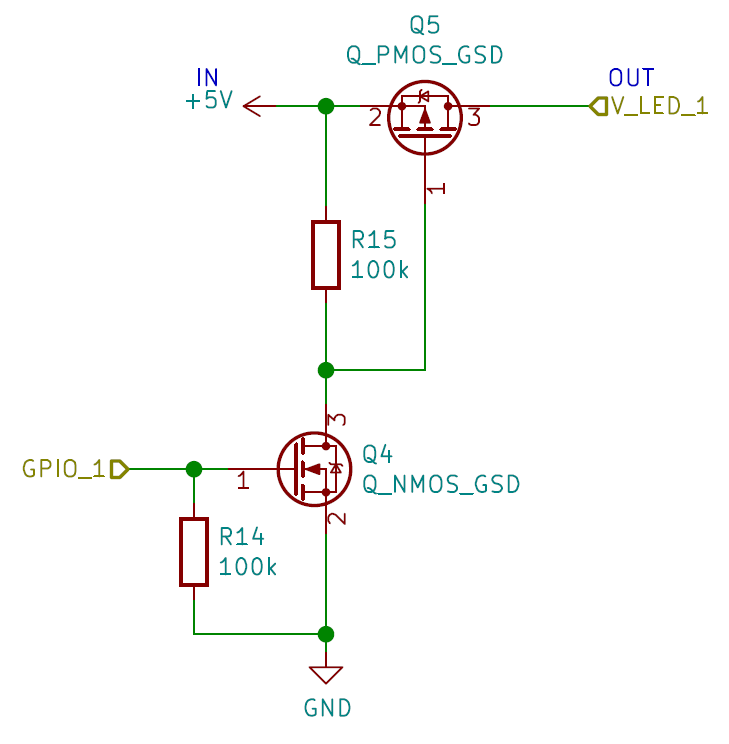
\includegraphics[scale=0.45]{obrazky/Zapinani_napajeni_LED.png}
    \end{center}
    \caption[Obvod pro zapínání napájení pro inteligentní LED]{Obvod pro zapínání napájení pro inteligentní LED.}
  \end{figure}

  Napájení inteligentních LED nelze spínat pouze jedním tranzistorem, protože logická~1~mikrokontroléru ESP32-PICO má hodnotu pouze 3,3~V. 
  V~tomto případě je ale zapotřebí spínat 5~V. Pokud by byl pro spínání použit pouze jeden tranzistor, tak by bylo napájení vždy sepnuto.

  Vstupně-výstupní pin mikrokontroléru ESP32-PICO je nastaven do logické~0. V~případě, že je zapotřebí rozsvítit další LED na řádku, který 
  nemá zapnuto napájecí napětí, tak je GPIO pin nastaven do logické~1 a~napájecího napětí je přivedeno dané skupině LED. 
  
  Při logické nule na gate 
  tranzistoru Q4 je tranzistor zavřený. Tranzistor Q5 v~tomto okamžiku drží zavřený rezistor R15.

  Když je signál GPIO\_1, přivedený z~mikrokontroléru, přepnut do logické~1, tak se tranzistor Q4 otevře. Otevřením tranzistoru Q4 je gate tranzistoru Q5 
  připojen ke GND a~tím se otevře i~tranzistor Q5, kterým je sepnuto napájecí napětí dané skupině inteligentních LED.

  Rezistor R14 udržuje tranzistor Q4 zavřený při nestandardních stavech pinu mikrokontroléru, jako je např. při resetu procesoru.

  \section{Mechanické prvky}
  Přepínač SW1 slouží pro zapínání celé DPS. Tento přepínač připojuje napájecí napětí 5~V~z~USB konektoru k~celému zbytku DPS. 

  Tlačítka SW2 až SW12 slouží pro ovládání hry. Ke každému tlačítku je připojen kondenzátor o~hodnotě 100~nF. Tento kondenzátor 
  slouží pro filtraci zákmitů při zmáčknutí tlačítka. Filtrace se díky tomu nemusí řešit softwarově.

  \begin{figure}[!h]
    \begin{center}
      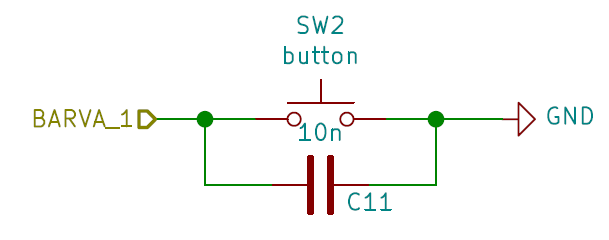
\includegraphics[scale=0.6]{obrazky/Tlacitka_zapojeni.png}
    \end{center}
    \caption[Zapojení tlačítek]{Zapojení tlačítek.}
  \end{figure}

  Přepínače SW13 až SW15 slouží pro volbu možnosti hry. První přepínač slouží pro volbu hry pro jednoho, nebo pro 2 hráče. Druhý 
  slouží pro možnosti hry na 3~nebo 4~herní prvky a~poslední přepínač slouží pro nastavení, zda se v~zadání může, nebo 
  nesmí vyskytnout mezera. 
  
  Z~důvodu obsazenosti pinů musely být přepínače připojeny k~mikrokontroléru ESP32 přes konfigurační piny. U~konfiguračních pinů
  musejí být dodržena pravidla pro připojovaná zařízení.
  Z~těchto důvodů je jeden přepínač připojen přes pulldown rezistor a~ostatní dva přepínače jsou připojeny přes pullup rezistor. 

  \begin{figure}[!h]
    \begin{center}
      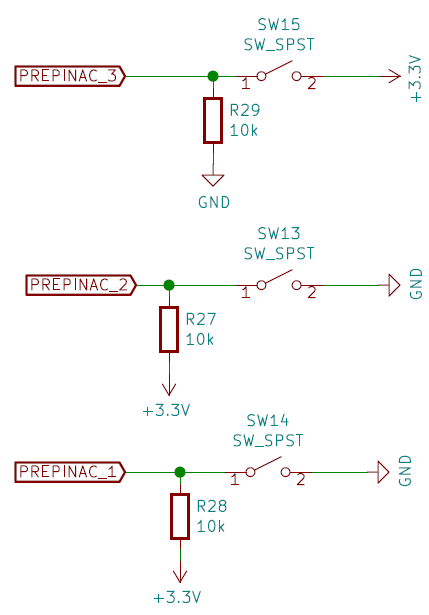
\includegraphics[scale=0.6]{obrazky/Prepinace_zapojeni.png}
    \end{center}
    \caption[Zapojení přepínačů]{Zapojení přepínačů.}
  \end{figure}

  \begin{table}[!h]
    \caption{Připojení přepínačů ke konfiguračním pinům mikrokontroléru ESP32-PICO}
    \begin{center}
        \begin{tabular}{|c|c|c|c|}
            \hline
            \rowcolor[HTML]{C0C0C0} 
            Přepínač   & Pin mikrokontroléru & Typ připojení rezistoru \\
            \hline
            SW14      & GPIO15 & Pullup \\
            \hline
            SW13      & GPIO05 & Pullup \\
            \hline
            SW15      & GPIO02 & Pulldown \\
            \hline
        \end{tabular}    
    \end{center}
  \end{table}

  \section{Indikace přítomnosti napájecího napětí}
  Pro indikaci přítomnosti napájecího napětí slouží LED~D1~a~D2. Elektroluminiscenční dioda~D1 indikuje přítomnost napájecího napětí 
  5~V~a~LED~D2 indikuje přítomnost napájecího napětí 3,3~V. Obě LED mají zelenou barvu a~jsou připojeny přes
  rezistor o~hodnotě 10~k$\Omega$.

  \begin{figure}[!h]
    \begin{center}
      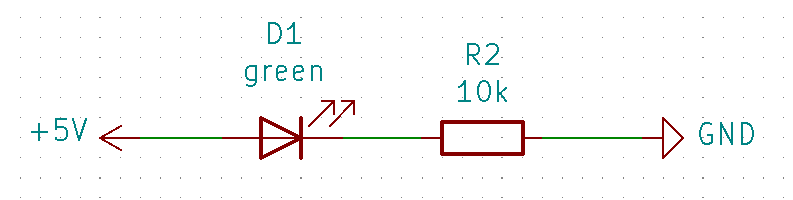
\includegraphics[scale=0.6]{obrazky/powerLED.png}
    \end{center}
    \caption[Zapojení LED pro indikaci napájecího napětí]{Zapojení LED pro indikaci napájecího napětí.}
  \end{figure}

  \chapter{Návrh DPS}
  Deska plošného spoje je navržena v~programu KiCad a~její parametry jsou určeny pro výrobu i~osazení ve firmě JLCPCB \cite{KiCad} \cite{JLCPCB}. Výrobní 
  podklady proto musely být navrženy v~souladu s~jejich výrobními možnostmi \cite{JLCPCB_Capabilities}.

  Deska plošného spoje má 4~vrstvy. Vnitřní vrstvy slouží pro napájení a~vnější pro signálové dráhy. V~jedné vnitřní vrstvě je po celé její ploše 
  polygon GND a~ve druhé vnitřní vrstvě jsou polygony jednotlivých napájecích napětí. Součástky jsou rozloženy tak, aby pokud možno
  korespondovaly s~polygony a~jednotlivá napájecí napětí tak nemusela být dále rozváděna zbytečně po celé DPS. Někdy však nemohlo být umístění 
  přizpůsobeno a~napájecí napětí tak muselo být přivedeno dráhou v~horní nebo spodní vrstvě, které jsou převážně určeny pro signálové 
  dráhy. 

  Na vrchní straně jsou umístěny plošky pro osazení součástek, protože firma JLCPCB osazuje součástky pouze z~jedné strany DPS.

  Signálové dráhy jsou vedeny úzkou dráhou a~napájecí dráhy jsou vedeny širší dráhou. V~signálových drahách tečou zanedbatelné 
  proudy, proto mohou být co nejužší. Výrobce umožňuje vyrobit u~čtyřvrstvé DPS nejtenčí dráhu 0,09~mm \cite{JLCPCB_Capabilities}. 
  Aby nebyly použity krajní výrobní hodnoty, byla zvolena šířka signálové dráhy 0,15~mm.

  Dráhy, kterými je vedeno napájecí napětí, mají tloušťku 0,5~mm. Pro výpočet šířky dráhy byla použita online kalkulačka Printed
  Circuit Board Width Tool \cite{Kalkulacka_drahy_DPS}. 
  Celá DPS obsahuje 84~inteligentních LED a každá z~nich má průměrný odběr proudu 5~mA. Celkový proudový odběr byl stanoven dle:

  \begin{equation} 
    I~=~I_{LED}~\cdot~n~=~5~\cdot~84~=~420~\:~mA.
  \end{equation}

  Proud dráhami při použití všech inteligentních LED je 420~mA a~tloušťka 
  mědi 35~$\mu$A \cite{JLCPCB_Capabilities}. Doporučená šířka dráhy byla tedy 0,236~mm, a~proto byla zvolena šířka dráhy 0,5~mm.

  Vnější vrstvy byly vyplněny polygonem GND. Zejména tak bylo učiněno kvůli výrobnímu procesu nanášení nepájivé masky. Tato maska
  může být velmi tenká zejména na plochách, kde jsou pouze tenké dráhy a~žádné velké plochy. Vytvoření polygonu GND tak dopomáhá
  k~vytvoření pevné a~stejně tlusté nepájivé masky. 

  \newpage
  \section{Vzhled DPS}
  Vzhled DPS byl ovlivněn vzhledem deskové hry a~výrobními možnostmi firmy JLCPCB. Rozměry DPS velmi ovlivňují cenu výroby. U~firmy 
  JLCPCB je zlomová hranice 10~$\times$~10~cm. Poté cena DPS rapidně narůstá. Rozměry 10~$\times$~10~cm byly pro návrh DPS Elektronické 
  hry Logic dostačující a~DPS byla tedy navržena na tyto rozměry. Poté byly do těchto rozměrů rozmisťovány součástky. 

  Inteligentní LED WS2812C jsou rozděleny do 3~skupin, aby se hra co nejvíce podobala deskové hře. Zároveň dopomáhá orientaci ve hře.
  Také kvůli množství inteligentních LED a~jejich poměrně velkým rozměrům (5~$\times$~5~mm) zabírají velkou část DPS 
  \cite{WS2812C_datasheet}. Proto musely být inteligentní LED rozmístěny jako první.

  Inteligentní LED pro zadání jsou umístěny v~horní části DPS. V~levém sloupci pod zadáním se nachází matice inteligentních LED, které slouží jako herní 
  pole, a~v~pravém sloupci je matice inteligentní LED pro vyhodnocení tahu. Rozložení LED reprezentuje herní tahy, proto jsou v~matici 4~$\times$~10~LED.
  
  Rozmístění tlačítek a~přepínačů probíhalo dle 
  rozmyšleného způsobu ovládání elektronické hry. Byl také brán ohled na estetiku vzhledu. Proto byly tlačítka i~inteligentní LED
  rozmístěny dle přesné mřížky. Následně byl ostatními obvody využíván zbylý prostor. 

  Dráhy s~napájecím napětím by měly být co nejkratší a~měly by být vedeny co nejvíce zpříma. Proto byla snaha o~umístění součástkek
  se stejným napájecím napětím k~sobě. Ne vždy ale mohla být tato doporučení splněna. Někdy musel být proveden kompromis mezi vzhledem a~funkčním 
  zapojením. 

  Dílčí obvody byly rozmístěny v~následujícím pořadí~-~USB konektory, měnič napětí, převodník z~USB 
  na RS-232 a~mikrokontrolér ESP32-PICO. Konektory USB musely být umístěny na okraj DPS, proto byly jednotlivé části obvodu naskládány podél levého okraje.

  Převodník úrovně je umístěn vždy těsně před vstupem signálu do první inteligentní LED daného řetězce.

  Přepínač pro změnu hry pro jednoho a~pro 2~hráče byl umístěn do mezery, mezi herními a~vyhodnocovacími inteligentními LED. Další 2~přepínače, jeden 
  pro volbu hry na 3~nebo 4~herní prvky a~druhý na volbu nastavení, zda se v~zadání může, nebo nesmí vyskytnout mezera, jsou umístěny v~pravém 
  horním rohu. 

  Obvody pro zapínání napájení jednotlivým sekcím inteligentních LED jsou umístěny vždy na začátku dané části polygonu vlevo od herních inteligentních
  LED.

  Vypínač pro zapínání napájení celé DPS je realizován kolébkovým vypínačem. Tento vypínač je umístěn na stěně krabičky a~pomocí drátových propojek 
  je připájen do připravených pájecích otvorů v~DPS.

  \section{Funkční rozmístění součástek}
  U~některých součástek není jejich umístění na DPS lhostejné. Rozmístění součástek v~některých případech může ovlivnit funkčnost obvodu. 
  Rozmístění součástek často souvisí s~rozkreslením ve schématu. Například kondenzátory filtrující šum napájecího napětí se umisťují co nejblíže přívodu 
  napájení.

  Rozložení součástek měniče napětí na DPS může velmi ovlivnit jeho funkčnost, zejména pak jeho účinnost. Proto bylo rozložení a~zapojení součástek 
  převzato z~datasheetu.

  \begin{figure}[!h]
    \begin{center}
      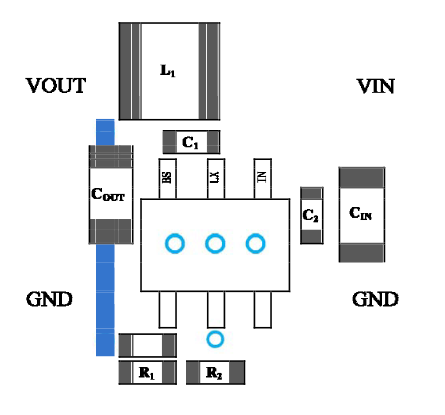
\includegraphics[scale=1]{obrazky/SY8105_rozlozeni_na_DPS.png}
    \end{center}
    \caption[Rozložení součástek kolem čipu SY8105 na DPS \cite{SY8105_datasheet}]{Rozložení součástek kolem čipu SY8105 na DPS 
    \cite{SY8105_datasheet}.}
  \end{figure}

  Signály D+~a~D- od konektoru USB k~čipu CP2102 jsou diferenciálním párem. Tomuto faktu musely být přizpůsobeny i~dráhy těchto signálů. Dráhy 
  jsou vedeny vedle sebe a~blízko u~sebe. Po celou jejich délku se nepřibližují ani neoddalují. Zkřížení probíhá až těsně před vstupem do čipu CP2102.
  Kondenzátory u~mikrokontroléru ESP32-PICO a~u~čipu CP2102 musí být umístěny co nejblíže jejich pouzdru. Tyto kondenzátory slouží pro 
  filtraci šumu na napájecím napětí. Stejná pravidla platí také pro filtrační kondenzátory u~inteligentních LED WS2812C.

  Kondenzátory u~tlačítek jsou také umístěny co nejblíže pouzdru tlačítek. Čím blíže pouzdru kondenzátor bude, tím lépe budou 
  filtrovány zákmity při stisku tlačítka.

  \chapter{Oživení DPS}
  Při výrobě finální verze DPS Elektronické hry Logic byly využity maximální možnosti osazení firmou JLCPCB.  
  Pro oživení finální DPS je tedy zapotřebí pájení pouze vypínače, který není umístěn na DPS, ale je zasazen do krabičky a~zapájen
  do DPS pomocí drátových prodlužek. 

  Při objednání finální DPS nastaly problémy s~nedostatkem součástek, se kterým se v~této době potýká mnoho návrhářů \cite{Nedostatek_soucastek}. 
  Čip SY8105 neměla firma JLCPCB dlouhodobě na skladě a~nebylo možné čekat, než jej budou znovu osazovat. Z~tohoto důvodu byl na finální DPS přeosazen 
  z~nefunkčních prototypů. Za klasických okolností by byl ale i~tento čip osazen firmou JLCPCB.

  Po připojení DPS přes USB konektor k~powerbance, nebo do počítače, se rozsvítí LED~D1 a~D2, které indikují přítomnost 
  napájecího napětí. Elektroluminiscenční dioda D1 značí přítomnost napětí 5~V~z~powerbanky a LED~D2 značí správnou funkci zapojení měniče napětí, tedy přítomnost 
  napětí 3,3~V.
  %odběr proudu

  \chapter{Od prvního prototypu po finální verzi}

  Před finální verzí byly navrženy 2~prototypy DPS elektronické hry Logic. Verze~0 byla pouze testovací, takže neobsahovala celé herní pole. 
  Sloužila pro ověření funkčnosti daných zapojení různých čipů a~zároveň pro základní testování softwaru.

  \begin{figure}[!h]
    \begin{center}
      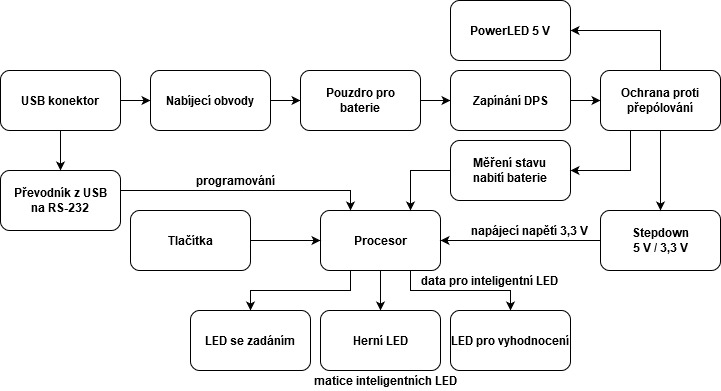
\includegraphics[scale=0.5]{obrazky/v0_blokove_schema.jpg}
    \end{center}
    \caption[Blokové schéma zapojení prototypu verze~0.0]{Blokové schéma zapojení prototypu verze~0.0.}
  \end{figure}

  \begin{figure}[!h]
    \begin{center}
      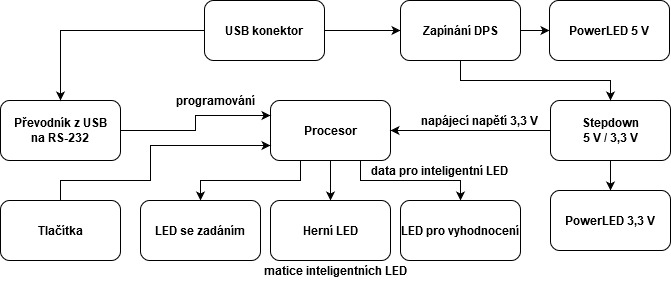
\includegraphics[scale=0.5]{obrazky/v1_blokove_schema.jpg}
    \end{center}
    \caption[Blokové schéma zapojení prototypu verze~1.0]{Blokové schéma zapojení prototypu verze~1.0.}
  \end{figure}

  Asi největším rozdílem mezi verzí prototypu~0.0~a~1.0 je způsob napájení. Verze~0.0 je napájena z~baterií a~verze~1.0 je napájena pomocí USB 
  konektoru. Díky této změně 
  odpadly i~mnohé části obvodu. Díky absenci baterií bylo možné odstranit nabíjecí obvody, ochranu proti přepólování a~měření napětí 
  na bateriích.       

  \section{Způsoby napájení prototypů}
  Každý z~prototypů měl velmi odlišný způsob napájení. V~následujících kapitolách je popsán způsob napájení prototypových verzí.

  \subsection{Verze~0.0}
  V~první verzi prototypu byly pro napájení použity baterie Li-Ion INR18650-29E od firmy Samsung. Tyto baterie mají jmenovité napětí 3,7~V, 
  při plném nabití až 4,2~V~\cite{18650}. Kapacita jedné baterie je 2850~mAh \cite{18650}. Byly použity 2~články baterií, které byly spojeny 
  paralelně. Paralelním zapojením byla celková kapacita zdvojnásobena.

  Baterie typu Li-Ion jsou náchylné na podvybití. Verze~0.0 proto obsahovala i~měření napětí na bateriích. Pokud by došlo k~podvybití, mohla 
  by se bateriím zmenšovat kapacita nebo by se mohly zničit. 

  \begin{figure}[!h]
    \begin{center}
      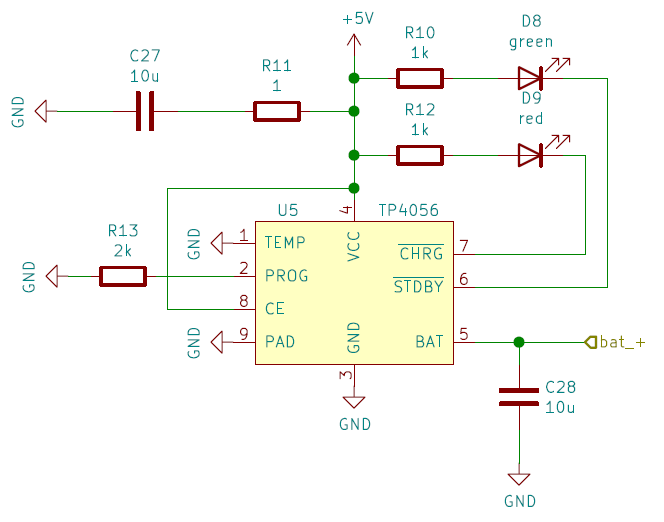
\includegraphics[scale=0.6]{obrazky/TP4056_schema.png}
    \end{center}
    \caption[Schéma zapojení čipu TP4056 \cite{TP4056_datasheet}]{Schéma zapojení čipu TP4056 \cite{TP4056_datasheet}.}
  \end{figure}

  Pro baterie bylo vybráno pouzdro na 2~články s~THT montáží do DPS \cite{18650_pouzdro}.

  Pouzdro s~bateriemi bylo připevněno a~zapájeno přímo do DPS, a~proto musel být integrován i~nabíjecí obvod. Nabíjení probíhalo přes konektor 
  USB~Micro.

  Pro nabíjecí obvod byl zvolen čip TP4056. Tento obvod byl vybrán, protože je přímo určen pro nabíjení baterií typu Li-Ion. Existují 
  moduly pro nabíjení těchto baterií, které mají integrovaný tento čip \cite{Nabijeci_modul}. Tyto moduly jsou často používané, a~proto 
  bylo zapojení tohoto modulu převzato do této práce. 

  Vlastnosti čipu jsou přizpůsobeny bateriím Li-Ion. Nabíjení baterií probíhá do 4,2~V, což je maximální napětí na použitých 
  bateriích \cite{18650} \cite{TP4056_datasheet}. Díky tomu nemůže dojít ke zničení baterií nabíjením.

  Červená LED~D9 indikovala nabíjení baterií a~zelená LED~D8 svítila, pokud byly baterie nabité \cite{TP4056_datasheet}. 
  Pokud nesvítila ani červená ani zelená LED, znamenalo to, že baterie jsou podvybité, nebo nejsou vloženy. Příčinou mohla být také příliš vysoká, 
  nebo nízká jejich teplota \cite{TP4056_datasheet}.

  Rezistorem R13 se určoval nabíjecí proud baterií \cite{TP4056_datasheet}. Aby baterie nabíjením nebyly poškozovány, měl by být nabíjecí 
  proud maximálně 0,5~C (polovina kapacity baterie). Vybraná baterie má kapacitu 2850~mAh. Nabíjecí proud proto mohl být až 1425~mA. 
  Jelikož je pro tuto hru důležitější kapacita baterie, než doba nabíjení, byl zvolen nabíjecí proud pouze 0,5~A. Čím menším proudem 
  je baterie nabíjena, tím má delší životnost a~pomaleji ztrácí svoji kapacitu.

  \begin{table}[!h]
    \caption{Nastavení nabíjecího proudu rezitorem R13 \cite{TP4056_datasheet}.}
    \begin{center}
      \begin{tabular}{|c|c|}
          \hline
          R13 [k$\Omega$] & Nabíjecí proud [mA] \\
          \hline
          10      & 130 \\
          \hline
          5       & 250 \\
          \hline
          4       & 300 \\
          \hline
          3       & 400 \\
          \hline
          2       & 580 \\
          \hline
          1,66    & 690 \\
          \hline
          1,5     & 780 \\
          \hline
          1,33    & 900 \\
          \hline
          1,2     & 1000 \\
          \hline
      \end{tabular}  
    \end{center}
  \end{table}

  Byl zvolen rezistor o~hodnotě 2~k$\Omega$, kterým byl určen nabíjecí proud 580~mA. 

  \newpage
  \subsection{Verze~1.0}
  Ve verzi~1.0 byl radikálně změněn způsob napájení. Napájení v~této verzi neprobíhá přes baterie, ale pouze přes USB konektor, přes 
  který ve verzi~0.0 probíhalo pouze nabíjení baterií. 

  Výhody
  \begin{itemize}
    \item absence drahých baterií,
    \item absence nabíjecího obvodu,
    \item absence hlídání stavu nabití baterie,
    \item absence ochrany proti přepólování (USB konektor je uzpůsoben svým tvarem, aby uživatel nemohl napájení přepólovat.),
    \item napájení inteligentních LED napětím přímo z~USB (Inteligentní LED mají menší odběr proudu.).
  \end{itemize}

  Nevýhody
  \begin{itemize}
    \item předpokládá se, že uživatel vlastní powerbanku,
    \item výdrž závisí na kapacitě powerbanky. 
  \end{itemize}

  Byl zvolen konektor USB~Micro, protože se jedná o~nejrozšířenější USB konektor dnešní doby.

  Do finální verze byl poté přidán ještě i~konektor USB-C.

  \subsection{Vývoj mechanických prvků}
  Na obou prototypech byla použita tlačítka s~THT montáží. Do finální verze byla použita tlačítka s~SMD montáží. Tato tlačítka jsou 
  robustnější a~celokovová. 

  Do finální verze byly přidány také přepínače pro volbu možností hry. 

  \section{Vzhled DPS}
  Prototyp verze 0.0 měl menší rozměry než finální verze. Sloužil pouze pro testování zapojení, odhalení nedostatků a~pro základní testování
  softwaru. 

  První prototyp také obsahoval pouzdro na baterie Li-Ion 18650, které bylo navrženo jako jediné na spodní straně DPS. Bylo tak umístěno
  kvůli úspoře místa. Rozmístění součástek základních dílčích obvodů bylo situováno především do horní části DPS. 

  Druhý prototyp se již svým vzhledem velmi podobal finální verzi.
  
  \section{Oživení prototypů}
  Při výrobě prototypů firma JLCPCB osazovala pouze SMD komponenty. Komponenty THT musely být doosazovány ručně. V~následujících kapitolách
  je popsán způsob oživování prototypů DPS.

  \subsection{Verze 0.0}
  Deska plošného spoje přišla z~výroby ve stavu, kdy byly osazeny pouze SMD komponenty.

  \begin{figure}[!h]
    \begin{center}
      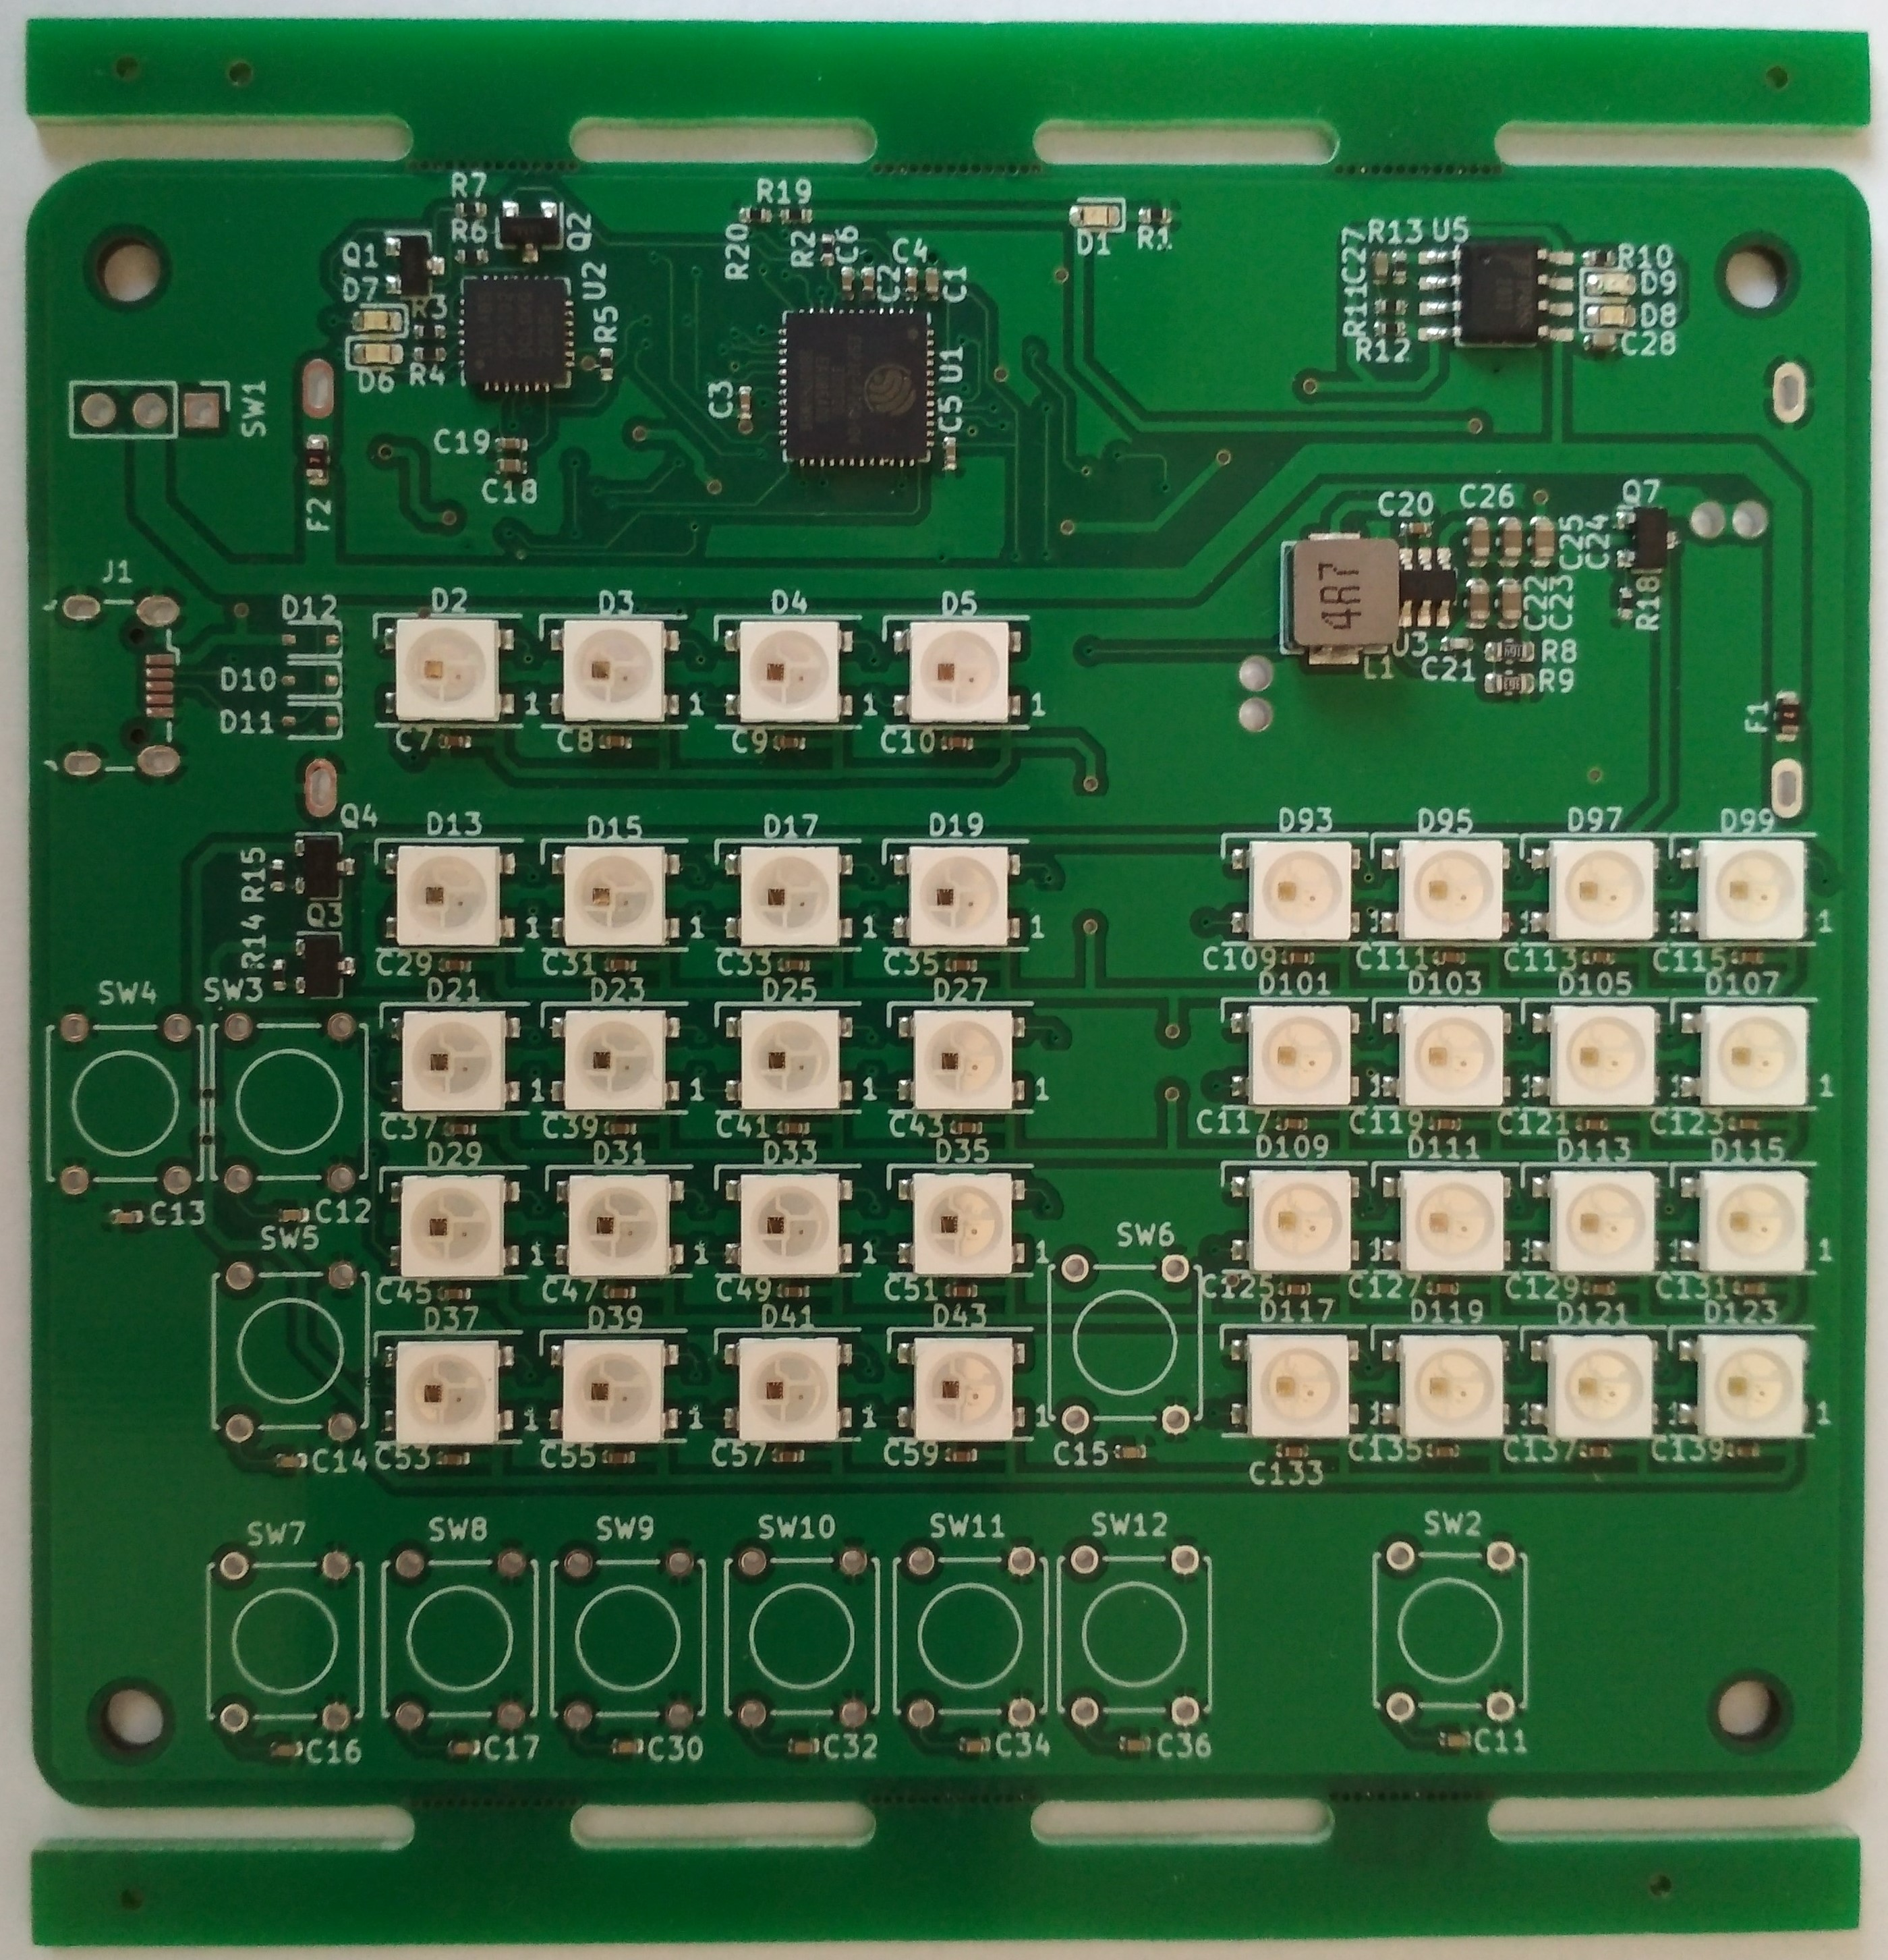
\includegraphics[scale=0.1]{obrazky/Verze0_vyroba_kolejnice.jpg}
    \end{center}
    \caption[DPS prototypu verze~0.0 z~výroby]{DPS prototypu verze~0.0 z~výroby.}
  \end{figure}

  Po dodání DPS z~výroby byly zapájeny THT komponenty (pouzdro na baterii, konektor USB Micro, tlačítka a~vypínač). Na testovací verzi
  byl místo vypínače osazen konektor, na který je pro zapnutí DPS potřeba nasunout propojku. Po zapojení baterií
  18650 do pouzdra a~zapnutí vypínače se rozsvítí zelená LED~D1, která indikuje přítomnost napájecího napětí. 

  Po vložení baterií do pouzdra a~zapnutí DPS bylo pomocí multimetru zjištěno, že ochrana proti přepólování baterií nepropouští napětí 
  dále, i~když jsou baterie v~pouzdře umístěny se správnou orientací napětí. Bylo zjištěno, že pouzdro tranzistoru zajišťujícího ochranu proti přepólování 
  neodpovídá navrženému pouzdru tranzistoru. Všechny MOSFET tranzistory byly stejného typu, takže musely být všechny odpájeny a~otočeny.
  
  Při zkoušce nabíjení bylo zjištěno, že červená LED indikující nabíjení baterií je přepólovaná. Elektroluminiscenční diodu se povedlo otočit a~indikace nabíjení 
  baterií z~USB byla v~pořádku. 
  
  Při programování byl zjištěn problém s~komunikací po lince RS-232. Bylo zjištěno, že zapojení LED pro indikaci komunikace po lince RS-232 bylo 
  chybně navrženo, a~proto byly LED odstraněny a~nahrazeny zkratem. Jejich zapojení této komunikaci bránilo. Do další verze byly překresleny správně.
  Bipolární tranzistory byly taktéž osazeny ve špatném pouzdře a~neodpovídaly navrženým pouzdrům. 
  
  Při programování a~testování všech inteligentních LED WS2812C a~tlačítek bylo zjištěno, že jedno tlačítko bylo zapojeno na pin, který 
  nemá softwarově zapínatelný pullup rezistor. Tento rezistor byl dodatečně osazen a~do schématu i~DPS další verze zakreslen. 
  
  Po veškerých opravách byla DPS plně funkční a~připravena na testování softwaru Elektronické hry Logic.

  \begin{figure}[!h]
    \begin{center}
      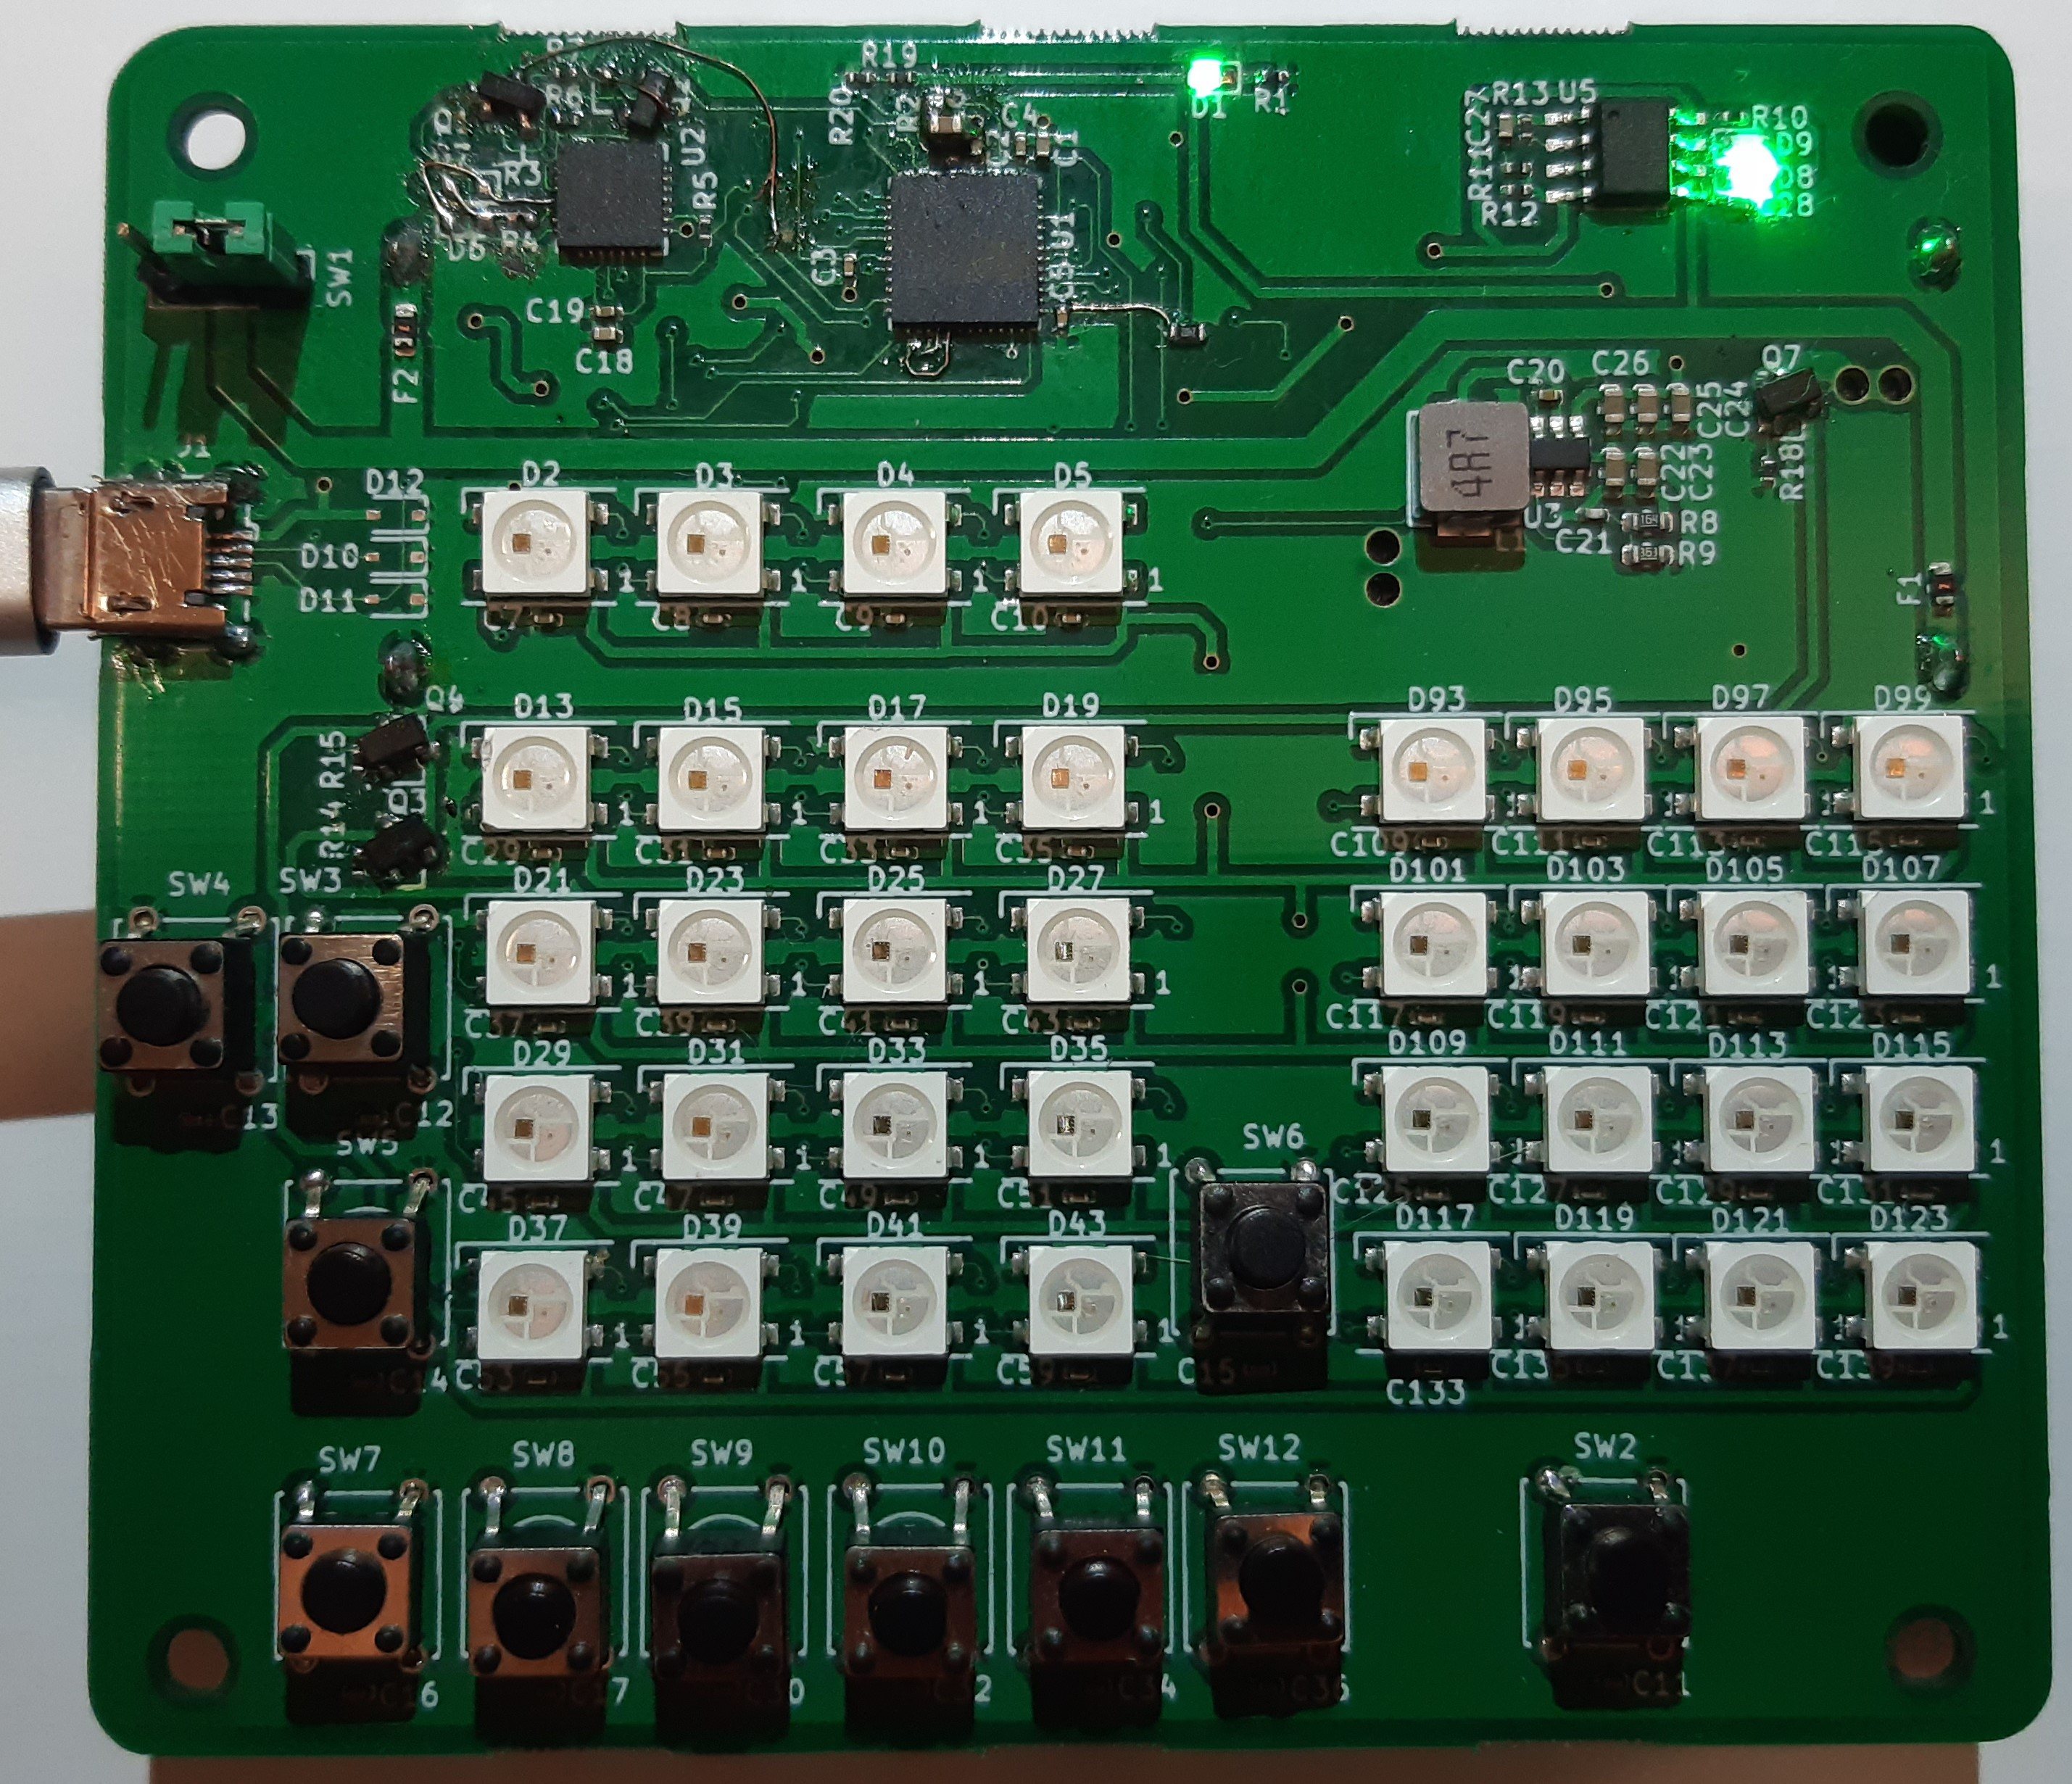
\includegraphics[scale=0.1]{obrazky/Verze0_zapnuto_nabito.jpg}
    \end{center}
    \caption[Oživená verze prototypu~0.0 s~opravami]{Oživená verze prototypu~0.0 s~opravami.}
  \end{figure}

  \newpage
  \subsection{Verze~1.0}
  Deska plošného spoje přišla z~výroby ve stavu, kdy byly osazeny pouze SMD komponenty. 

  \begin{figure}[!h]
    \begin{center}
      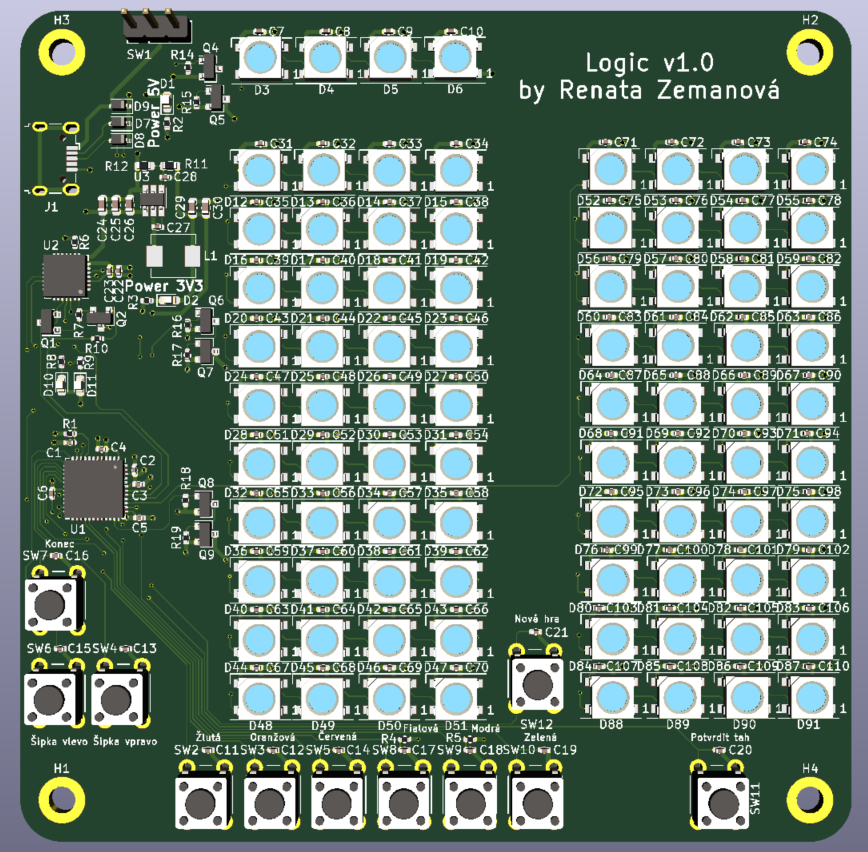
\includegraphics[scale=0.65]{obrazky/Verze1_3D_pohled.png}
    \end{center}
    \caption[3D~pohled DPS prototypu verze~1.0]{3D~pohled DPS prototypu verze~1.0.}
  \end{figure}

  Poté byly ručně osazeny THT součástky, tj. vypínač, tlačítka a~konektor USB Micro. Po připojení DPS přes USB konektor k~powerbance, 
  nebo do počítače, se rozsvítí LED~D1~a~D2, které indikují přítomnost napájecího napětí. LED~D2 zároveň značí, že zapojení měniče
  napětí je funkční.

  Všechny chyby z~předchozí verze prototypu byly odstraněny. Deska plošného spoje byla tedy plně funkční a~mohla být programována hra Logic v~plném rozsahu.
  
  Po otestování byly k~DPS přidány přepínače a~poté byla finální verze DPS objednána.

  

 
  




